\documentclass[aspectratio=169]{beamer}
\usetheme{Madrid}
\usecolortheme{default}

\title[APSM Gossip Learning]{Decentralized Edge Workload Forecasting\\using Semantic Gossip Learning and Agentic AI}
\subtitle{Mid-Semester 1 Evaluation}
\author[P. Mungra]{Parthkumar Mungra\\(2022IMT-082)}
\institute[ABV-IIITM]{
    Supervisor: Dr. Mahendra Kumar Shukla\\
    \vspace{0.2cm}
    Integrated Master of Technology in IT\\
    ABV-IIITM Gwalior
}
\date{\today}

\begin{document}

\begin{frame}
    \titlepage
\end{frame}

\begin{frame}{Presentation Outline}
    \tableofcontents
\end{frame}

\section{Introduction}
\begin{frame}{Introduction \& Motivation}
    \begin{columns}
        \begin{column}{0.35\textwidth}
            \begin{itemize}
                \item \textbf{Edge Computing:} Moving compute close to IoT devices.
                \item \textbf{DFaaS:} Decentralized Serverless Functions.
                \item \textbf{Goal:} Proactive load forecasting to prevent edge failures.
            \end{itemize}
        \end{column}
        \begin{column}{0.65\textwidth}
            \begin{figure}
                \centering
                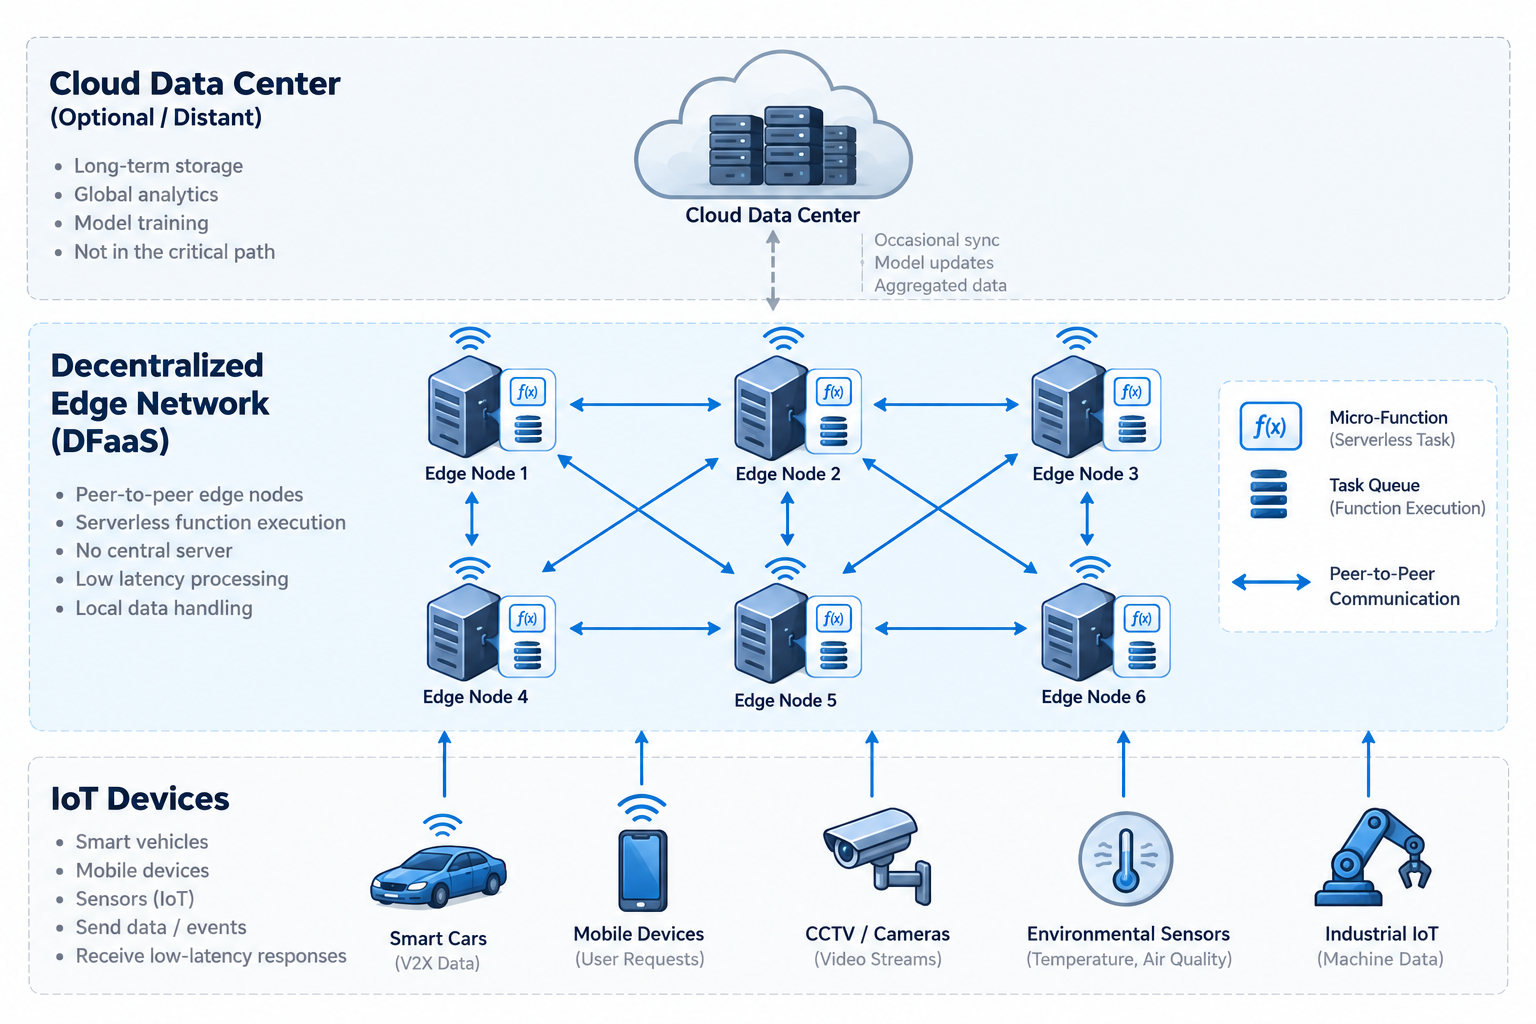
\includegraphics[width=\textwidth]{figures/edge_architecture.png}
                \caption{Decentralized Edge Architecture}
            \end{figure}
        \end{column}
    \end{columns}
\end{frame}

\section{Background}
\begin{frame}{Background: Federated vs. Gossip Learning}
    \begin{columns}
        \begin{column}{0.35\textwidth}
            \begin{itemize}
                \item \textbf{Federated Learning:} Centralized aggregator (Single point of failure).
                \item \textbf{Gossip Learning (GL):} Fully decentralized, peer-to-peer.
                \item \textbf{Why GL?} Unmatched fault tolerance.
            \end{itemize}
        \end{column}
        \begin{column}{0.65\textwidth}
            \begin{figure}
                \centering
                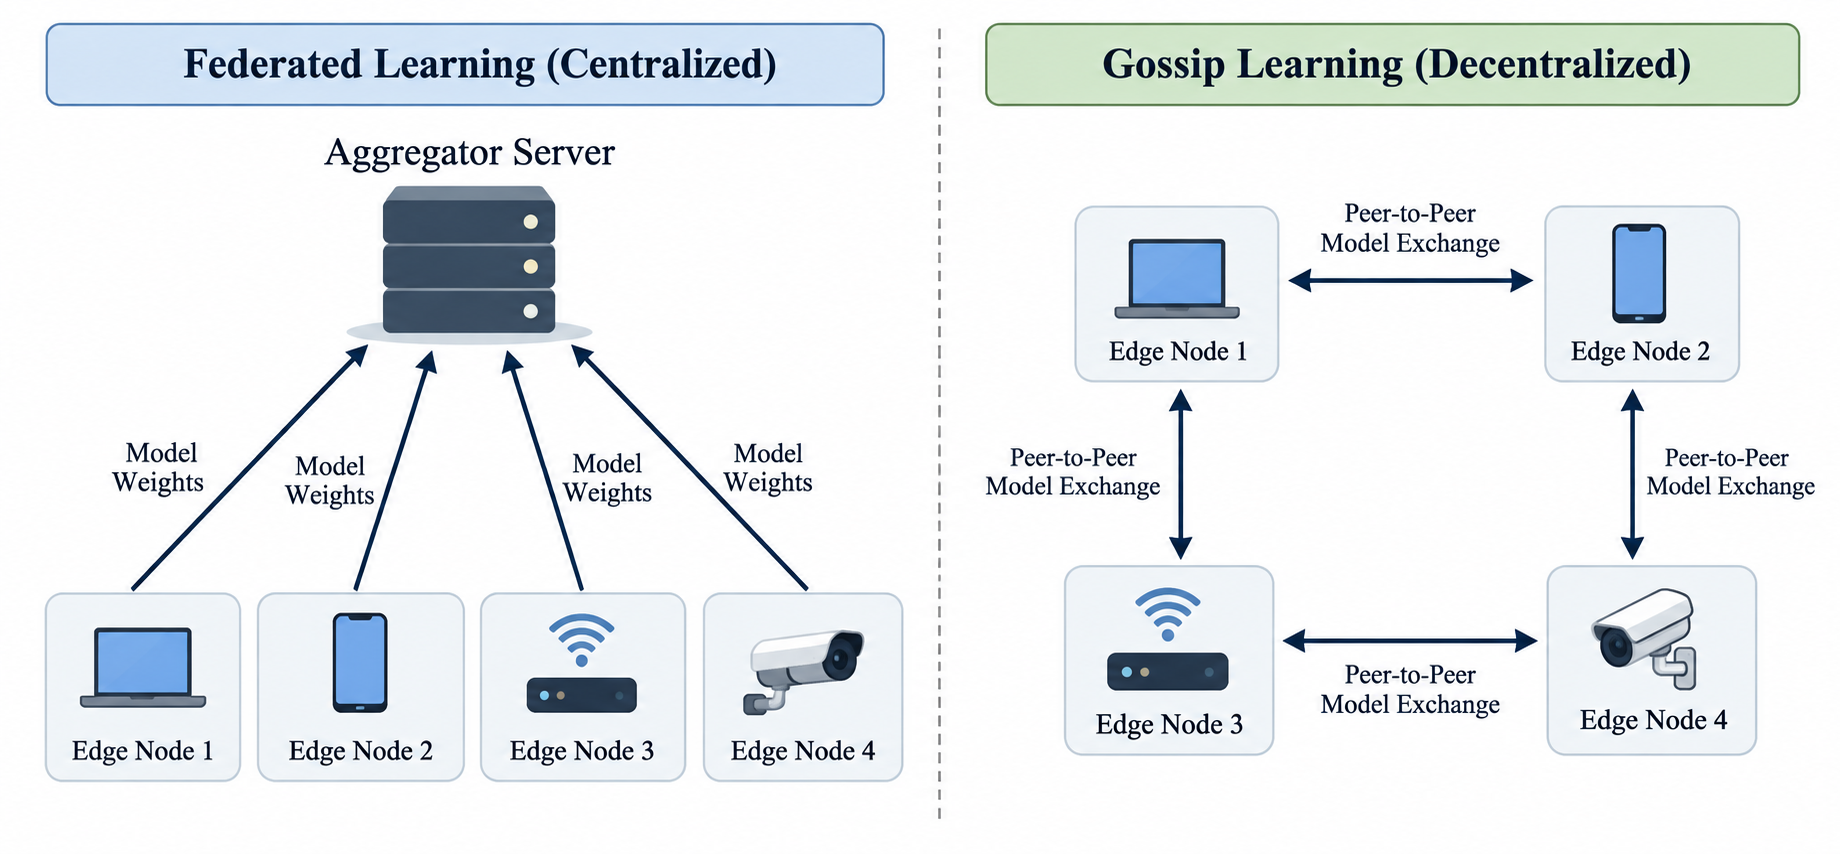
\includegraphics[width=\textwidth]{figures/fl_vs_gl.png}
                \caption{FL vs. GL Topology}
            \end{figure}
        \end{column}
    \end{columns}
\end{frame}

\section{Problem Statement}
\begin{frame}{The Core Problem: Gossip Learning Inefficiencies}
    \begin{itemize}
        \item \textbf{The Issue:} Standard GL transmits massive neural network models on a rigid, continuous schedule.
        \vspace{0.3cm}
        \item \textbf{Negative Impacts:}
        \begin{itemize}
            \item Severe wireless bandwidth saturation.
            \item Unnecessary CPU merging cycles.
            \item Rapid battery depletion on edge nodes.
        \end{itemize}
        \vspace{0.3cm}
        \item \textbf{Objective:} Build a smart filter that stops redundant model transmissions without hurting accuracy.
    \end{itemize}
\end{frame}

\section{Proposed Solution}
\begin{frame}{Proposed Solution: The APSM Framework}
    \begin{columns}
        \begin{column}{0.35\textwidth}
            \begin{itemize}
                \item \textbf{APSM Filter:} Evaluates model's "Semantic Value".
                \item \textbf{Rule:} Only transmit if prediction is a "surprise".
                \item \textbf{Result:} Predictable traffic = No transmission.
            \end{itemize}
        \end{column}
        \begin{column}{0.65\textwidth}
            \begin{figure}
                \centering
                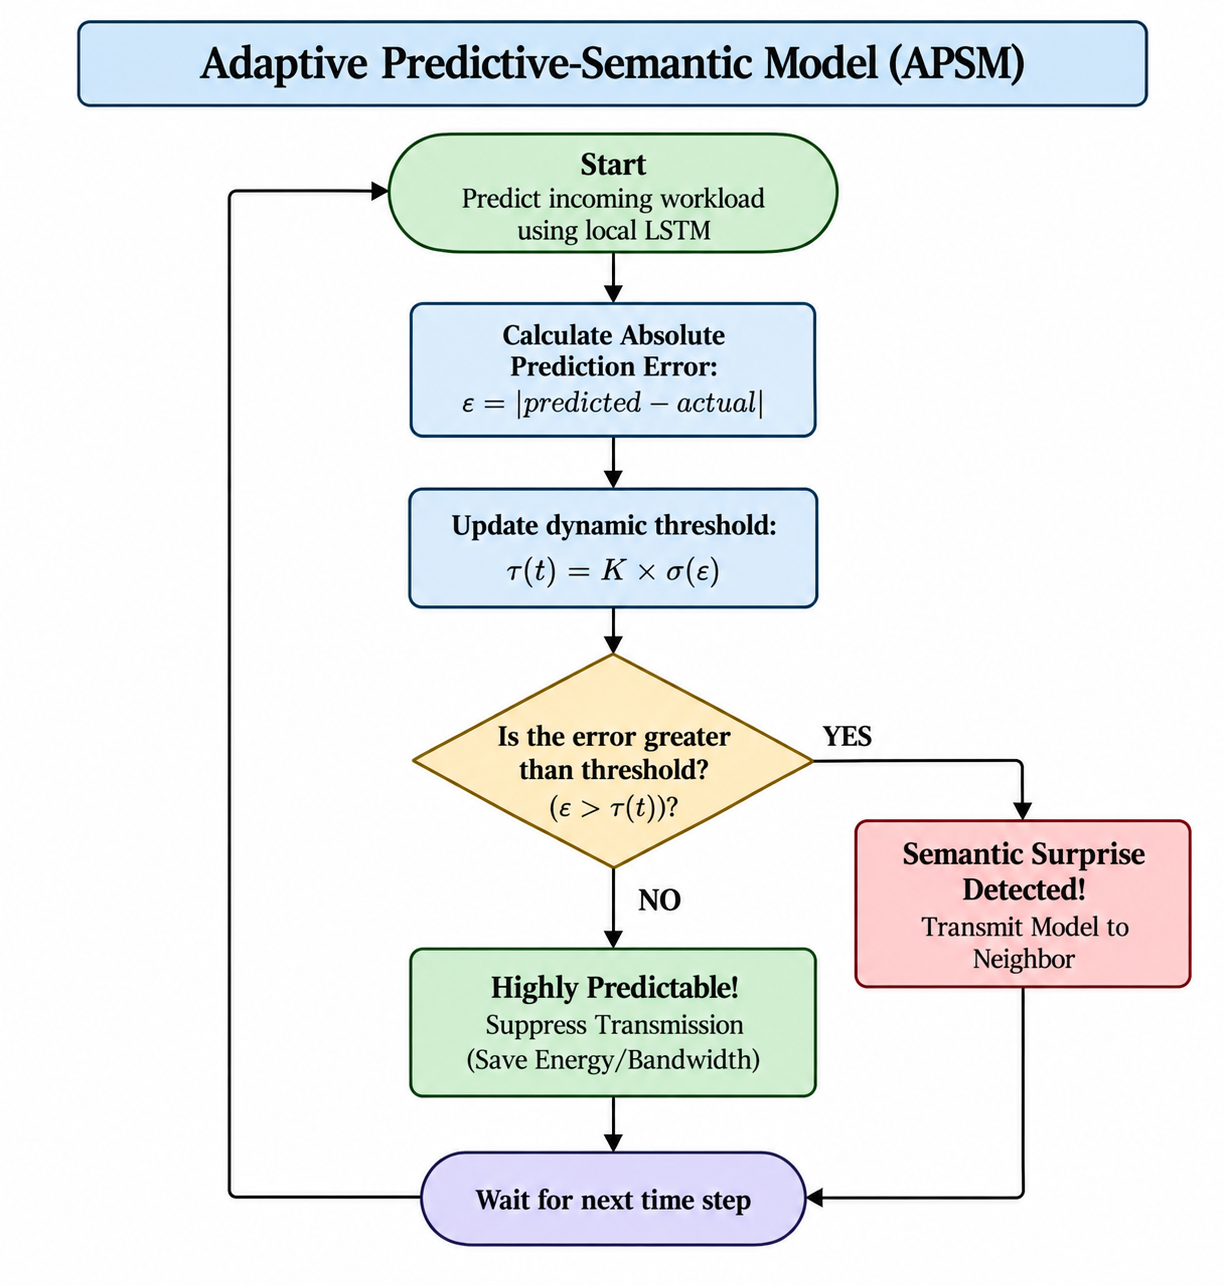
\includegraphics[width=\textwidth]{figures/apsm_workflow.png}
                \caption{APSM Logic Flowchart}
            \end{figure}
        \end{column}
    \end{columns}
\end{frame}

\begin{frame}{Mathematical Methodology}
    \begin{columns}
        \begin{column}{0.5\textwidth}
            \textbf{Absolute Prediction Error ($\epsilon$):}
            \begin{equation}
                \epsilon(t) = | y(t) - \hat{y}(t) |
            \end{equation}
            \vspace{0.3cm}
            
            \textbf{Adaptive Threshold ($\tau$):}
            \begin{equation}
                \tau(t) = K \times \sigma(\epsilon)
            \end{equation}
            (Where $K = 2.0$, $\sigma =$ standard deviation)
        \end{column}
        \begin{column}{0.5\textwidth}
            \textbf{Semantic Suppression Rule:}
            \vspace{0.3cm}
            \begin{itemize}
                \item $\epsilon(t) > \tau(t)$ \\
                $\rightarrow$ \textbf{Transmit Model}
                \vspace{0.3cm}
                \item $\epsilon(t) \leq \tau(t)$ \\
                $\rightarrow$ \textbf{Suppress Model}
            \end{itemize}
        \end{column}
    \end{columns}
\end{frame}

\section{Results}
\begin{frame}{Experimental Setup (Phase 1)}
    \begin{itemize}
        \item \textbf{Simulator:} Custom discrete-event edge network simulator.
        \item \textbf{Topology:} 10-Node, 3-edge-connected peer-to-peer network.
        \item \textbf{Dataset:} Microsoft Azure serverless traces + Porto taxi mobility.
        \item \textbf{Model:} Local Univariate LSTM (1 hidden layer, 16 units).
    \end{itemize}
\end{frame}

\begin{frame}{Results: Bandwidth \& Energy Savings}
    \begin{columns}
        \begin{column}{0.4\textwidth}
            \begin{itemize}
                \item \textbf{Bandwidth Reduced:} 49.61\%
                \item \textbf{Energy Saved:} 49,710 Joules (13 Wh)
                \item \textbf{Impact:} Network congestion literally cut in half.
            \end{itemize}
        \end{column}
        \begin{column}{0.6\textwidth}
            \begin{figure}
                \centering
                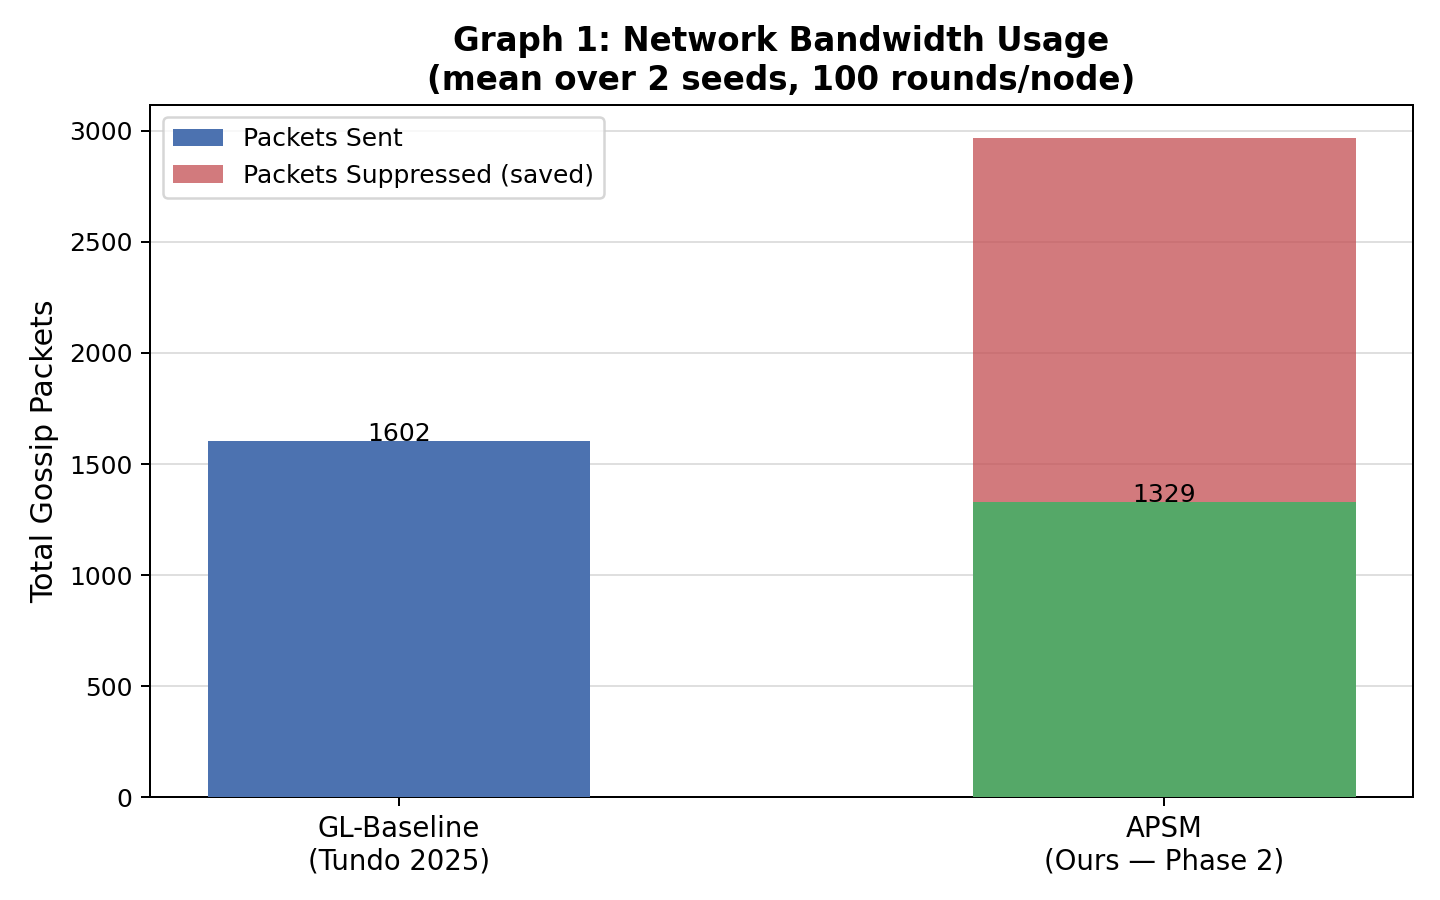
\includegraphics[width=\textwidth]{figures/10n_graph1_bandwidth.png}
                \caption{Bandwidth Reduction}
            \end{figure}
        \end{column}
    \end{columns}
\end{frame}

\begin{frame}{Results: Forecasting Accuracy Preservation}
    \begin{columns}
        \begin{column}{0.4\textwidth}
            \begin{itemize}
                \item \textbf{Challenge:} 50\% suppression usually ruins accuracy.
                \item \textbf{APSM Result:} Only 4.50\% MSE degradation.
                \item \textbf{Why?} Critical "surprises" are always broadcasted.
            \end{itemize}
        \end{column}
        \begin{column}{0.6\textwidth}
            \begin{figure}
                \centering
                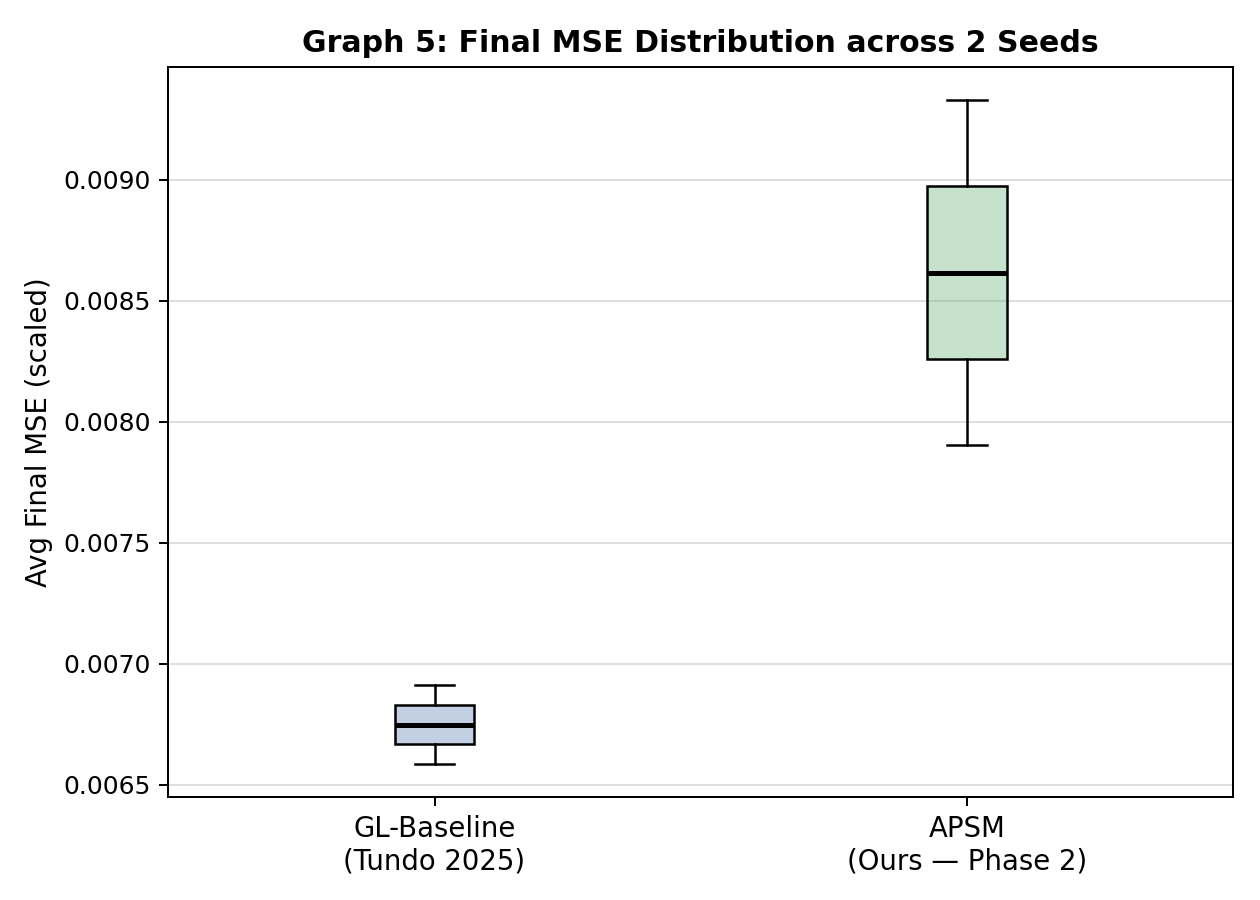
\includegraphics[width=\textwidth]{figures/10n_graph5_mse_boxplot.png}
                \caption{MSE Distribution Boxplot}
            \end{figure}
        \end{column}
    \end{columns}
\end{frame}

\section{Future Scope}
\begin{frame}{Future Plans (Semester 2)}
    \begin{columns}
        \begin{column}{0.35\textwidth}
            \begin{itemize}
                \item \textbf{Scaling up:} 50 \& 100 node networks.
                \item \textbf{Agentic AI:} Deploy autonomous agents to actively negotiate offloading.
            \end{itemize}
        \end{column}
        \begin{column}{0.65\textwidth}
            \begin{figure}
                \centering
                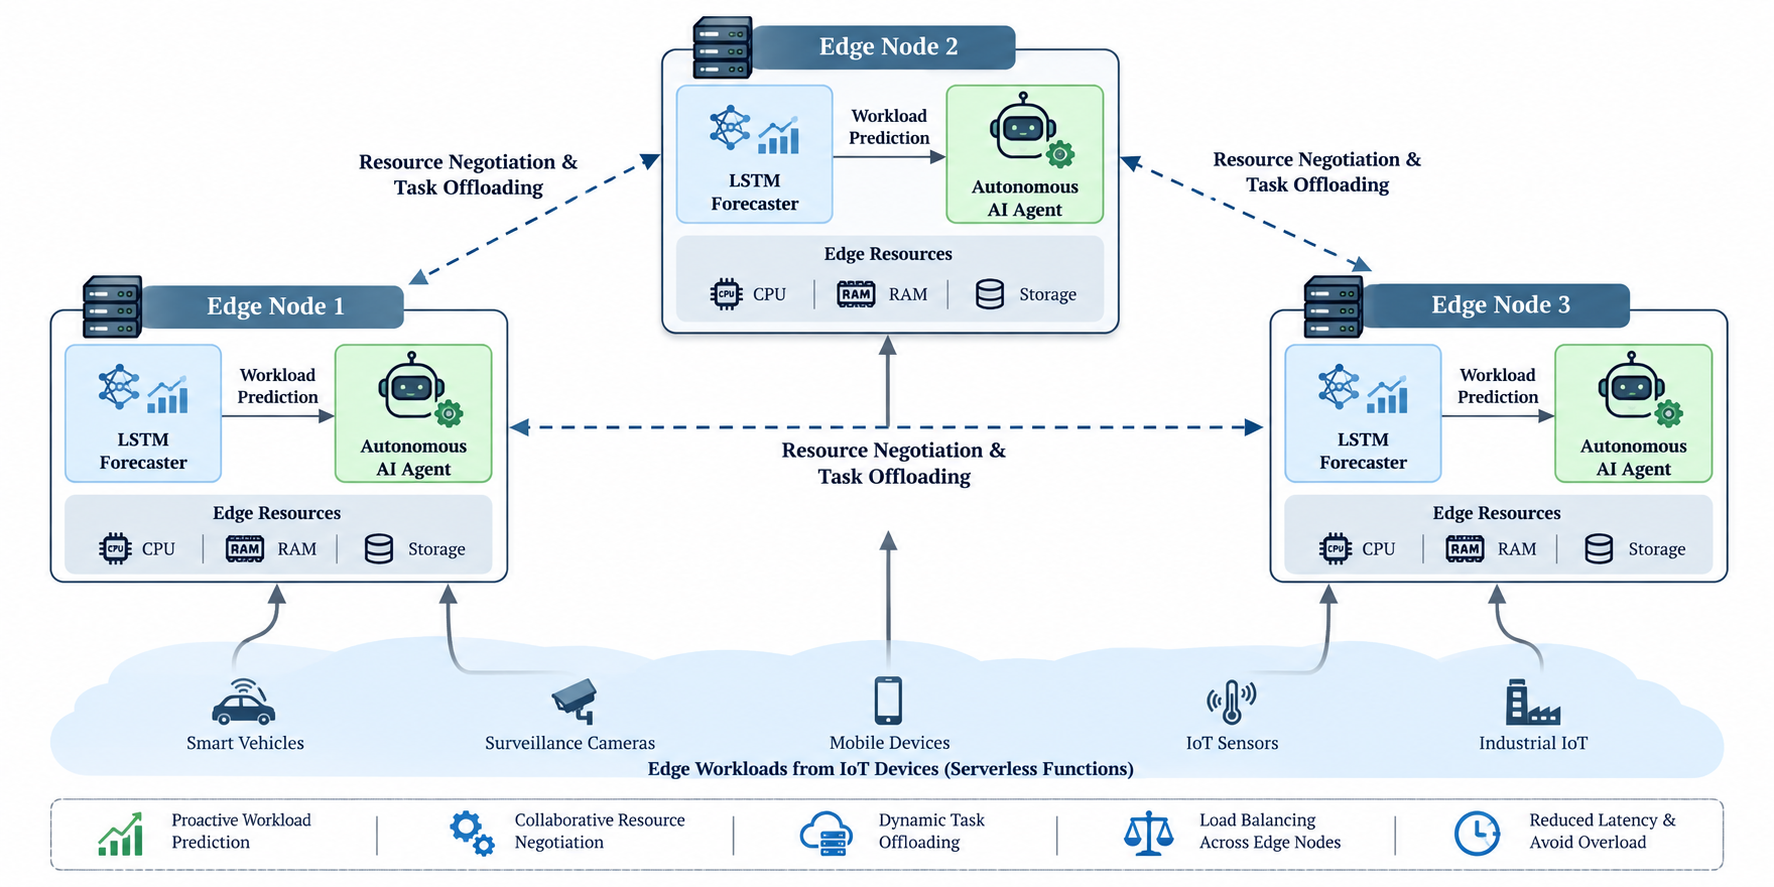
\includegraphics[width=\textwidth]{figures/agentic_ai.png}
                \caption{Agentic AI Roadmap}
            \end{figure}
        \end{column}
    \end{columns}
\end{frame}

\section{References}
\begin{frame}{Key References}
    \begin{itemize}
        \item \textbf{[1] Gossip Learning:} A. Tundo \textit{et al.}, "Decentralized Edge Workload Forecasting with Gossip Learning," \textit{IEEE International Conference on Edge Computing}, 2025.
        \item \textbf{[2] Agentic AI:} G. Yao, H. Liu, and L. Dai, "Multi-Agent Reinforcement Learning for Adaptive Resource Orchestration in Cloud-Native Clusters," \textit{ICDA}, ACM, 2025.
    \end{itemize}
\end{frame}

\begin{frame}
    \centering
    \Huge \textbf{Thank You!}
    
    \vspace{1cm}
    \Large Questions?
\end{frame}

\end{document}
